\documentclass[letterpaper, 10 pt, conference]{ieeeconf}
                                                      

\IEEEoverridecommandlockouts                            
\overrideIEEEmargins
% See the \addtolength command later in the file to balance the column lengths
% on the last page of the document

\usepackage{epigraph}
\usepackage{booktabs}
\usepackage{graphicx}
\usepackage{fancyvrb}
\usepackage{fancyhdr}
\usepackage{lastpage}
\usepackage{amsmath}

% The following packages can be found on http:\\www.ctan.org
%\usepackage{graphics} % for	 pdf, bitmapped graphics files
%\usepackage{epsfig} % for postscript graphics files
%\usepackage{mathptmx} % assumes new font selection scheme installed
%\usepackage{times} % assumes new font selection scheme installed
%\usepackage{amsmath} % assumes amsmath package installed
%\usepackage{amssymb}  % assumes amsmath package installed

\title{\LARGE \bf
Major League Baseball Hall of Fame Classification with Principal Component Analysis*
}

\author{Christopher Hua$^{1}$, Joseph Maher$^{2}$, and Raghav Joshi$^{3}$
\\University of Pennsylvania
\\2 May 2015 % <-this % stops a space
\thanks{*Prepared for STAT 471/701 (Spring 2015), with Professor Linda Zhao.}% <-this % stops a spac
\thanks{$^{1}$ Contact Christopher at {\tt\small chua@wharton.upenn.edu }}% 
\thanks{$^{2}$ Contact Joseph at {\tt\small maherj@wharton.upenn.edu}}%
\thanks{$^{3}$ Contact Raghav at {\tt\small raghav.joshi.15@gmail.com}}%
}

\begin{document}

\maketitle
\thispagestyle{plain}
\pagestyle{plain}

%%%%%%%%%%%%%%%%%%%%%%%%%%%%%%%%%%%%%%%%%%%%%%%%%%%%%%%%%%%%%%%%%%%%%%%%%%%%%%%%
\begin{abstract}

Each year, the Baseball Writers’ Association of America (BBWAA) elects players into the Hall of Fame. While many statistics are collected about players, induction into the Hall of Fame remains difficult to predict. In this paper, we present three different classifiers to predict whether or not a given player will make the Hall of Fame, evaluated on the basis of cross-validated error. We find that logistic classification with principal components had the best predictive power, and a regular logistic model was second best. We also consider tradeoffs between interpretability and accuracy. Finally, we consider the applications of our models and research.

\end{abstract}


%%%%%%%%%%%%%%%%%%%%%%%%%%%%%%%%%%%%%%%%%%%%%%%%%%%%%%%%%%%%%%%%%%%%%%%%%%%%%%%%
\section{INTRODUCTION}

\epigraph{``If Jesus Christ were to show up with his old baseball glove, some guys wouldn't vote for him. He dropped his cross three times, didn't he?''}{\textit{Dick Young, former president of the Baseball Writers Association of America}}

Perhaps no debate in Major League Baseball is fiercer than the yearly squabble about who should be inducted into the Baseball Hall of Fame, the  highest honor in the game. The annual vote by the Baseball Writers Association of America (BBWAA) and the Major League Baseball Veteran's Committee is therefore the source of constant controversy among fans, players, writers, managers and statistics students alike. 

Hall of Fame voters consider a large number of factors, including quantitative factors, such as a player's career home runs, runs batted in or on-base percentage, as well as qualitative factors such as a player’s character or his most iconic moments. 

In recent years, the debate about who to elect has become a de facto referendum on different approaches to assessing player value. Sabermetrics, as popularized by \textit{Moneyball}, now have a first-class role in baseball. Many observers argue that these advanced metrics should play a larger role in determining a player's election into Cooperstown. However, others counter that a player's true worth cannot be quantified and other factors, such as success in big games, character or intangibles must also be considered. 

Though it is clear that voters take different measures into account when filling out their ballots, it is not clear which factors are most important or who will be elected. This study will examine voting trends for hitters elected to the Hall of Fame and build a classifier of who will be elected. This will allow us to better understand what qualities make a Hall of Fame player.

We present three models:
\begin{enumerate}
\item Logistic Regression
\item Logistic Regression on Principal Components
\item Random Forest
\end{enumerate}

We compare the three models in terms of interpretability, robustness, and prediction accuracy. We then apply our final model to predict the results of upcoming Hall of Fame ballots.

\section{DESCRIPTION OF THE DATA}
We created a comprehensive dataset of all baseball players with major league appearances, along with many of their career statistics. The data is drawn from two primary sources: Sean Lahman's database of baseball statistics and Baseball Reference’s daily Wins Above Replacement (WAR) calculation dump. As a note, there are two competing measures of WAR: the BBRef version we used, also known as rWAR, and FanGraphs’ version, known as fWAR. Over a large set of data, the difference between the two measures is miniscule. We include instructions to build the dataset in the appendix.

The {{\tt\small Lahman }} dataset is complete up until 2013. We refrained from making changes to the dataset because we want to ensure that any such changes are done in a consistent matter. We only make one change - to fix a typo in a player's ID.

The cleaning and analysis were done solely in R. We made heavy use of the {{\tt\small reshape2 }}and {{\tt\small dplyr}} packages in cleaning the data. We use the {{\tt\small ggplot2}} and {{\tt\small reshape}} packages for some of the fancy graphics. We use the {{\tt\small boot}}, {{\tt\small tree}}, {{\tt\small randomForest}}, and {{\tt\small class}} packages while creating classifiers. 
\subsection{Subsetting Data}
Our primary dataset is of modern-era batters. We chose to define this dataset as being players who retired between 1950 and 2000 , who were primarily position players, and had at least 10 years of service. We do this for several reasons:
\begin{itemize}
\item Post-war play is generally considered the modern era – we want to look at the period that most accurately reflects our current baseball playing field, no matter how much Rob Manfield wants to change it. The focus on professionalism also arises during this period.
\item It becomes exceedingly difficult to separate pitchers and hitters in early baseball data. We could buld a classifier for this, but because so many players played at both positions anyways, it’s kind of a moot point. See the appendix for a comparision of pre- and post-war players and their at-bats per year. There is a fairly clear divide at 120 at bats per year as being the divide between pitchers and batters. 
\item A number of included variables are simply not recorded in early baseball. These include All-Star Game appearances (began 1933), Gold Glove awards (began 1957), sacrifice hits, and a couple others. 

We thus limit the years in order to accurately reflect the leverage of these variables on the dataset.
\item All players who retired after 2000 were still eligible for the Hall of Fame as of the 2014 ballot (the last covered in the Lahman dataset). We want to ignore these players as well as any active players because they haven’t had all their chances to be elected to the Hall of Fame yet. 

\item Because ballplayers must have at least 10 years of service in the majors to be elected to the Hall of Fame, we also include that as a requirement. As a result, our training body of data better reflects the pool of players that could be nominated for the ballot.


\end{itemize}

It should be noted that cutting off the dataset in the year 2000 limits the exposure of this dataset to baseball's Steroid Era. Many players who are suspected or admitted steroid users have been on the Hall of Fame ballot in recent years but have received very little support despite having outstanding statistical profiles. For example, every one of our models predicts that Barry Bonds has almost a 100 percent chance of election, but he has yet to receive more than 40 percent of the vote on a Hall of Fame ballot. There are several other notable outliers like this. By limiting the dataset to players who retired before 2000, we effectively eliminate the vast majority of these cases, which preserves the integrity of the dataset. However, it should be noted that prediction for future voting is more difficult due to the fact that there are so many players who have fallen under the cloud of steroid suspicion. Many players that our models predict for the Hall of Fame have extenuating circumstances casting shadows upon their candidacy.  

Our final working dataset has 887 observations of 39 variables. Unless otherwise noted, we broke our dataset into 75\% training data and 25\% test data. The sets that we use are consistent across all the models built.

\subsection{Included Variables}
Please see Table 1 for information about the 39 included variables. Of these, we often exclude the first 2 (player name and database player id) in our analyses. These variables shouldn't make a difference for our intended observation. This leaves 37 variables to consider.
\begin{table}[h]
\caption{Explanation of Variables}
%\label{my-label}
\centering
\begin{tabular}{@{}rl@{}}
\toprule
Variable Name & Description                   \\ \midrule
"playerName"  & Government name               \\
"playerID"    & Common key                    \\
"numYears"    & Years played                  \\
"lastYear"    & Last year appeared            \\
"g"           & Games appeared in             \\
"ab"          & At bats                       \\
"r"           & Runs scored                   \\
"h"           & Hits                          \\
"x2b"         & Doubles                       \\
"x3b"         & Triples                       \\
"hr"          & Home Runs                     \\
"rbi"         & Runs Batted In                \\
"sb"          & Stolen Bases                  \\
"cs"          & Caught Stealing               \\
"bb"          & Walks                         \\
"so"          & Strike-outs                   \\
"ibb"         & Intentional walks             \\
"hbp"         & Hit by pitch                  \\
"sh"          & Sacrifice hits                \\
"sf"          & Sacrifice flies               \\
"gidp"        & Grounded into double plays    \\
"totalWAR"    & Wins above replacement, BBRef \\
"totalInn"    & Total innings                 \\
"mvp"         & \# of MVP awards              \\
"gg"          & Golden Gloves                 \\
"sisl"        & Silver Sluggers               \\
"tc"          & Batting Triple Crown          \\
"asgApp"      & All-Star Game appearances     \\
"inducted"    & In the HOF?                   \\
"pa"          & Plate appearances             \\
"obp"         & On-base percentage            \\
"ops"         & OBP + Slugging                \\
"slg"         & Slugging percentage           \\
"rc"          & Runs Created                  \\
"bAvg"        & Batting average               \\
"aby"         & At bats per year              \\
"threeK"      & At least 3000 hits?           \\
"fiveHundo"   & At least 500 HR?              \\
"threeHundo"  & At least 0.300 average?       \\ \bottomrule
\end{tabular}
\end{table}

\subsection{Data Exploration}
Faced with a lot of data and not a whole lot of idea of how to proceed, we explored the data in several dimensions.

First, we plotted the correlation matrix for our 37 variables in Figure 1.

\begin{figure}[thpb]
\centering
\framebox{\parbox{3in}{
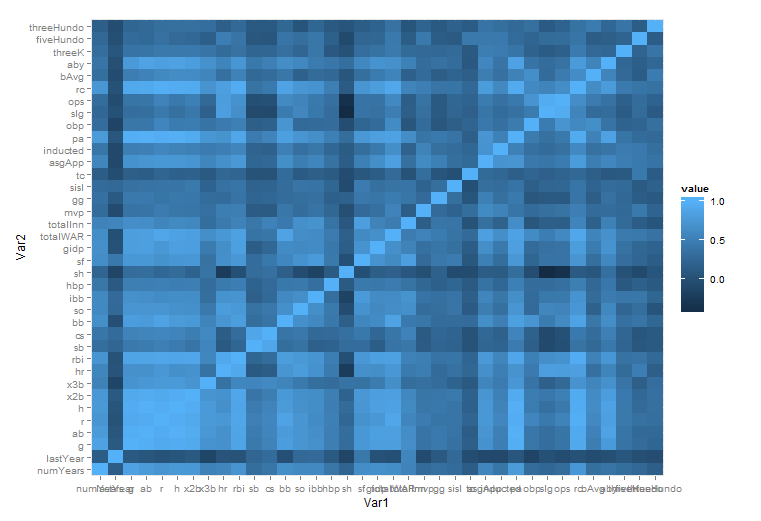
\includegraphics[width=3in]{cor.png}}}
\caption{Correlation table for modern batters dataset. See appendix for link to full-size version.}
\label{figurelabel}
\end{figure}

A few observations:
\begin{itemize}
\item The count data (hits, at bats, etc) are all closely correlated. This makes sense – the more at bats and plate appearances a player has, the more hits, runs, etc he is likely to have. 
\item We inserted a couple of dummy variables, such as “at least 3000 hits.” These qualitative benchmarks are of course tightly correlated with their counting stat counterpart.
\item Some of the rarer variables are not correlated with any others, which makes sense given how rare they are (e.g. Triple Crown of batting average, runs batted in, and home runs).
\item The {{\tt\small lastYear}} stat isn’t tightly correlated with any other variable, which is what we hoped to see. This means that there are no (obvious) non-linear effects of time. It is perhaps most tied with stolen bases, caught stealing, and sacrifice flies. This is expected because  recordkeeping for these statistics was inconsistent before the 1970’s.
\end{itemize}

We will explain more in depth later what principal component analysis (PCA) is, but plotting principal components against each other is an easy way to quickly visualize if there are particular trends to consider. Plotting the first two principal components versus each other gives a very interesting look into the subsets present within the data, as shown in Figure 2.

\begin{figure}[thpb]
\centering
\framebox{\parbox{3in}{
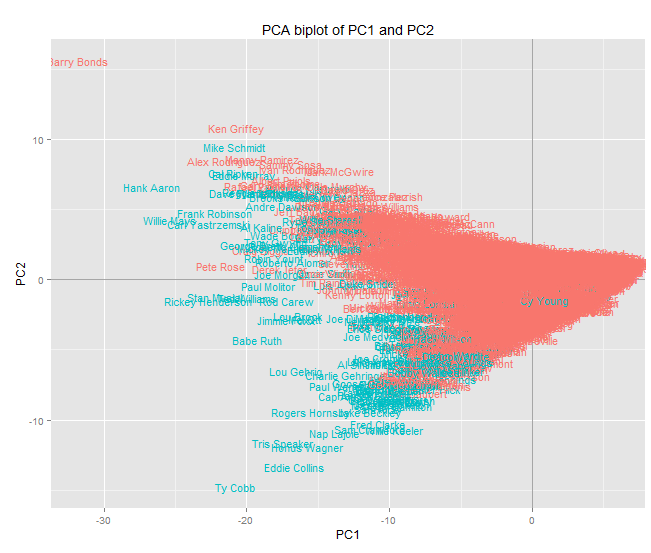
\includegraphics[width=3in]{pcabiplot.png}}}
\caption{Biplot of the first two principal components on the full batters dataset (no restriction on era). See appendix for link to full-size version.}
\label{figurelabel}
\end{figure}

This PCA biplot is useful for seeing various players’ deviances from the mean performance of hitters.\footnote{We provide code to plot the first 3 principal components as well, although the resulting graphs are not very useful to read in print.} We use the full set of players for this particular graph (including actives). A ‘truly average’ player would come in at (0, 0). In general, Hall of Fame players (in blue) are very far away from the mean. This lines up with our intuition – baseball’s Hall of Fame is notorious for selecting only the most outstanding players. These are the ones who are farthest from the mean. Let’s look at some of the most notable outliers:

\begin{itemize}
\item Barry Bonds and Pete Rose: Bonds and Rose are two of the all-time greatest hitters, and their separation from the rest of the points shows that in this graph. Bonds in particular destroys this graph – being beyond an all-time great power hitter, young Bonds was super-fast: a fielding monster with one the best Ultimate Zone Ratings and a speed demon on the bases. Since our model focuses on career totals, he gets insane leverage for his absurd counting stat totals – all-time leader in home runs, walks, intentional walks, career MVP shares, and second in WAR. Rose, likewise, had an excellent career with counting stats: all-time leader in hits, games played, at-bats, and singles. Barry Bonds is also literally why we can’t add single season statistics to this analysis – he got on base more times his second best season than he had at bats. Both of these players would be first-balloters – if it were not for their steroids and gambling scandals. 
\item Cy Young, Joe McGinnity, Vic Willis, Mickey Welch: At first glance, it’s kind of shocking to see any Hall of Fame players who played worse than average! Then it becomes clear that all of these players are pitchers. Our primary focus was modern batters for this analysis, and our classification for that was a relatively simple 120 plate appearances per year linear boundary. These 4 pitchers are old-timers who saw comparatively many plate appearances; they don’t affect our analysis proper since they were excluded from the “modern” dataset.
\item (Many) modern-era players: many of these players have great arguments for the Hall of Fame, but their reigns atop the batting tables are all accompanied with an asterisk -- allegations of steroid use are difficult for voters to overlook. 
\item Jimmy Sheckard, Bill Dahlen, Sherry Magee: These are the non-inducted players with the highest deviation from the mean in the positive direction of PC2. Notably, all three of these players were among those that Bill James pointed out as Hall of Fame snubs; traditional sabermetrics and our fun little modern statistical experiment agree yet again!
\end{itemize}

\section{LOGISTIC REGRESSION}
Logistic regression is a logical starting point because, albeit simple, it allows us to see which specific variables were significant in determining Hall of Fame election. Furthermore, the results are especially open to interpretation. The other models we used in this analysis merely give us classification while logistic regression enables us to look at specific probabilities for each player on the ballot

\subsection{Building a logistic classifier}
To build a logistic classifier, we started by incorporating all the variables in the dataset into one model. We then used backwards selection to reduce the included features, with a threshold of $p \leq 0.05$. In the end, we include a mere three variables: total Wins Above Replacement (WAR), the number of Golden Gloves won, and the number of All-Star Game appearances. The output is shown in figure 3, and the equation for the log-odds is shown below:

$$ln(\frac{p}{1-P})= -9.39 + 0.10 \times WAR - 0.28 \times GG + 0.57 ASG$$

\begin{figure}[thpb]
\caption{Final Logistic Regression Model}
\begin{Verbatim}[frame=single]
Call:
glm(formula = inducted ~ totalWAR + gg 
+ asgApp, family = binomial(logit), 
data = train) 
Deviance Residuals: 
  Min     1Q     Median     3Q    Max  
-3.8085 -0.0714 -0.0279  -0.0162 2.4509  

Coefficients:
            Estimate Std. Error Pr(>|z|)  
Intercept   -9.38672    1.30995 7.74e-13
totalWAR     0.10241    0.02167 2.30e-06
gg          -0.28226    0.12202 0.0207 
asgApp       0.56906    0.12880 9.96e-06
 
Null deviance: 318.68  on 664
degrees of freedom
Residual deviance:  83.95  on 661  
degrees of freedom
AIC: 91.95
 
Number of Fisher Scoring iterations: 9
\end{Verbatim}
\end{figure}

\subsection{Analysis of logistic classifier}
With only three inputs, the logistic classifier is very parsimonious and reasonably easy to interpret.

It is interesting that the number of Gold Gloves won has a negative coefficient. This means that, holding WAR and All-Star appearances constant, earning more Gold Gloves means a player is less likely to be inducted into the Hall of Fame. This could be because fielding prowess has historically been less important to voters than hitting. Because WAR incorporates measures of both fielding and hitting, players that earn Gold Gloves and thus a certain WAR value due primarily to fielding are not as successful in entering the Hall of Fame as those that earn that same WAR due to primarily to hitting. The model thus incorporates a negative value for Gold Gloves as a way to suss out the extent to which a player's WAR is determined by his fielding.

It is also noteworthy that out of all the variables in the dataset, only three are significant. This likely implies that WAR is a good proxy for most other relevant statistics in determining player value. Perhaps the most well known estimator of Hall of Fame chances, the JAWS model, uses only WAR as a predictor of Hall of Fame chances.\footnote{JAWS is an acronym for Jaffe WARP Score system, developed by sabermetrician Jay Jaffe. This model multiplies a player's career WAR by his seven year peak WAR, and compares the value to the average for HOF players at the same position.} 

All-Star Game appearances is the third variable that is a significant factor in this model at the 5 percent level. This statistic initially may seem highly collinear with lots of hitting statistics and WAR. However, All-Star Game appearances could help explain the difference between perception and reality. Similar to the Hall of Fame process, players are voted into the All-Star Game, invoking some element of popularity. This is especially true because starters are voted in by fans. Factors that may not necessarily show up in a box score or even in advanced metrics can influence All-Star voting just as these factors can influence Hall of Fame voters. Therefore, All-Star appearances can differentiate the perception of two players with otherwise identical statistical profiles.

We can now look at the model's effectiveness by making a classification table using the testing data. We found that the cutoff for induction of any player with a probability greater than 0.5 was the best way to minimize the error of this model.

\begin{table}[ht]
\centering
\caption{Test confusion matrix - Logistic classifier}
%\label{my-label}
\begin{tabular}{l|l|l|}
\cline{2-3}
                        & N   & Y  \\ \hline
\multicolumn{1}{|l|}{0} & 205 & 4  \\ \hline
\multicolumn{1}{|l|}{1} & 1   & 12 \\ \hline
\end{tabular}
\end{table}

The model gives us a misclassification rate of .023. This means that the model correctly predicted a player's Hall of Fame chances at a rate of .977. For fun, the player the model predicts would be in the Hall of Fame who is actually not enshrined is Rocky Colavito

We used 10-fold cross validation to check the accuracy of this model and found a prediction error of 0.0391, representing the average testing error of this model. This can be used to compare our different models.

\section{PRINCIPAL COMPONENT ANALYSIS}
The goal of principal component analysis (PCA) is to reduce the dimensionality of the data while preserving as much variance as possible. We take our set of (possibly) correlated variables, and transform them into a set of linearly uncorrelated variables. Principal components are chosen such that they maximize the variance present in the data, with the constraint that the given components are uncorrelated. Each principal component is a linear fit of the entire variable set. 

PCA is especially well suited to creating a classifier for the MLB Hall of Fame, because the method helps find hidden relationships in the data and helps detect outliers. Dimensional analysis helps us sift through our rich layers of data to find tiny nuggets of information. Additionally, great ballplayers are by definition outliers (Gladwell 08). As seen in figure 2, even 2 principal components are enough to start seeing how subsets align themselves in the data. Thus, PCA can help us with visualizing how players are separated while also creating a parsimonious model. 
\subsection{PCA and Classification with Training-Test}
We use the built-in {{\tt\small prcomp}} method to build a principal component analysis on the training data.
Figure 4 gives the output of the first 6 principal components.
\begin{figure}[thpb]
\caption{Importance of top 6 principal components}
\begin{Verbatim}[frame=single]
                          PC1     PC2
Standard deviation     4.2913 1.86654
Proportion of Variance 0.4977 0.09416
Cumulative Proportion  0.4977 0.59188
                           PC3     PC4
Standard deviation     1.57080 1.31934
Proportion of Variance 0.06669 0.04704
Cumulative Proportion  0.65856 0.70561
                           PC5     PC6
Standard deviation     1.24636 1.15456
Proportion of Variance 0.04198 0.03603
Cumulative Proportion  0.74759 0.78362
\end{Verbatim}
\end{figure}

The rest of the output is available in the appendix. Kaiser's criterion (Kaiser 1960) suggests keeping only the principal components that have eigenvalues of at least 1, of which we have 6. \footnote{We keep only factors that explain as much variation as the equivalent as one original variable.} Additionally, we examined the scree plot of this output (see appendix) and found a leveling off of eigenvalues after six components as well. To preserve parsimony, we also tested the model with 5 principal components. We found that the Akaike information criterion (AIC) was minimized with 6 principal components.

Functionally, this means that our dataset has been reduced from 37 dimensions to only 6, while still maintaining 78.36\% of the associated variance.
\subsection{Building the PCA Classifier}
We fit a generalized linear model on these 6 components to the training dataset. We then use the model to create a prediction index on the testing dataset.

\begin{figure}[thpb]
\centering
\framebox{\parbox{3in}{
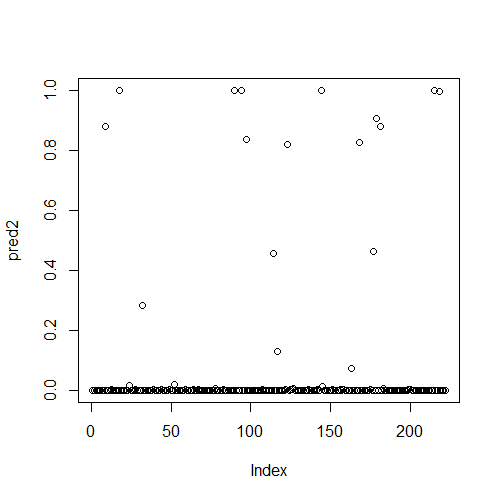
\includegraphics[width=3in]{predValues.png}}}
\caption{Prediction index values from principal component classifier. See appendix for link to full-size version.}
\label{figurelabel}
\end{figure}

Looking at this plot, we note that the vast majority of predicted values are very nearly 0, with a number above 0.8, and only a few in the middle. This is in-line with our expectations; we should see most players have virtually no shot at the Hall of Fame, and out of the players who have at least moderate chances at the Hall, a good number who are very likely to get in with only a few in the middle. 

\subsection{Analysis of PCA Classifier}

We found that the best boundary was to "induct" players with predicted values of at least 0.2. We should expect a similarly lower prediction boundary; as the common maxim goes, "if you have to make a case for them, they don't belong in the Hall of Fame." Table II shows the resulting confusion matrix, with 3 misclassified players out of 222 possible.

\begin{table}[ht]
\centering
\caption{Test confusion matrix - PCA classifier}
%\label{my-label}
\begin{tabular}{l|l|l|}
\cline{2-3}
                        & N   & Y  \\ \hline
\multicolumn{1}{|l|}{0} & 205 & 2  \\ \hline
\multicolumn{1}{|l|}{1} & 1   & 14 \\ \hline
\end{tabular}
\end{table}

For fun, we look at which players are misclassified. Our model thinks that Gary Carter and Kirby Puckett don't belong in the Hall of Fame, while it thinks that Roger Maris deserves a bust in Cooperstown. 

\section{RANDOM FOREST CLASSIFIER}

Random forests are another commonly used statistical learning method for classification, especially for datasets with a large number of parameters. The random forest method is a non-parametric ensemble learning algorithm that builds upon the weaknesses of decision trees. Because decision trees involve greedy and recursive partitioning, they manage to avoid overfitting the data, but at the same time, decision tree predictions have high bias and high variance.

Random forests combats the high variance problem through bagging which aggregates independently trained multiple bootstrap samples and then decreases test error using squared error loss. The process reduces the bias by comparing many different trees.

Thus, random forests are advantageous because they are highly accurate and remain interpretable. They're also faster to train, can handle larger numbers of predictors and do not require cross validation because the algorithm continually generates an internal estimate of the test error.

\subsection{Growing the Random Forest} 
We built the random forest with all possible explanatory variables for induction, and 10 possible variables sampled at each try. We also tell the model to check for importance of predictors, running it in supervised mode.

\subsection{Analysis of the Random Forest}
An important consideration is the importance of variables in the random forest. See appendix for a variable importance plot or see Table III for numerical results.

\begin{table}[ht]
\caption{Variable Importance Table for Random Forest}
%\label{my-label}
\centering
\begin{tabular}{@{}rl@{}}
\toprule
Variable   & Mean Gini Decrease \\ \midrule
totalWAR   & 12.67231007        \\
r          & 11.71652600        \\
rc         & 10.25806893        \\
asgApp     & 9.61028133         \\
rbi        & 5.77645975         \\
ab         & 2.90388928         \\
pa         & 2.54635874         \\
ops        & 2.19181570         \\
h          & 1.89536523         \\
hr         & 1.87136055         \\
slg        & 1.77473037         \\
aby        & 1.74836862         \\
g          & 1.70261248         \\
sh         & 1.43733553         \\
obp        & 1.30671964         \\
mvp        & 1.28764272         \\
x2b        & 1.14090090         \\
lastYear   & 1.12123952         \\
ibb        & 0.96456722         \\
sf         & 0.89126685         \\
totalInn   & 0.88703951         \\
bAvg       & 0.84545050         \\
bb         & 0.67953190         \\
x3b        & 0.62001074         \\
so         & 0.58467579         \\
numYears   & 0.51541444         \\
cs         & 0.48579664         \\
gidp       & 0.46279008         \\
hbp        & 0.45234404         \\
sb         & 0.42895584         \\
gg         & 0.28966631         \\
sisl       & 0.05906953         \\
threeHundo & 0.05043847         \\
threeK     & 0.03261879         \\
fiveHundo  & 0.01027273         \\
tc         & 0.00000000         \\ \bottomrule
\end{tabular}
\end{table}

The Gini coefficient is a measure calculated for each variable when the model considers a split for a node, which gives a measure of the heterogeneity accounted for by the variable, similarly to principal component values. We consider the variable importance later when comparing the random forest and straight logistic regression methods.

This method, however, underperforms the previously seen PCA classification method (Table 4) and the Logistic Regression (Table II). With the same testing and training data, the random forest mispredicts 8 players, compared to the PCA classifier's 3. Further, the random forest drastically underpredicts the number of observed responses; almost half of Hall of Fame players in the test set are misclassified. 

\begin{table}[h]
\centering
\caption{Confusion Matrix - Random forest classifier}
%\label{my-label}
\begin{tabular}{l|l|l|}
\cline{2-3}
 & Y & N \\ \hline
\multicolumn{1}{|l|}{0} & 205 & 1 \\ \hline
\multicolumn{1}{|l|}{1} & 7 & 9 \\ \hline
\end{tabular}
\end{table}

\section{COMPARISON OF METHODS}
	
	First and foremost, the comparison of the sensitivity rates (calculated from confusion matrices) show a different result than was expected. In most cases, ensemble methods such as random forests tend to be more accurate in predictive power (low bias and low variance) than logistic regression, but it doesn't seem to be the case here, especially when cross-validated. The logistic regression had 1 false positive and 4 false alarms, whereas the random forest had 7 false positives and 1 false alarm. The advantage of logistic regression is that there are simple probabilistic values for prediction compared to the use of scaled orthogonal eigenvectors found in PCA. Logistic regression also is favorable in the eyes of frequentists because it's easy to compute confidence intervals and is strong for categorical variables. One problem that can face logistic regression models is the level of the threshold (different threshold levels, subject to interpretation of the person creating the model, can produce different results i.e a 0.5 threshold is not as stringent as 0.75 threshold for Hall of Fame induction) and the linear separability that is apparent in regularization of logistic regression.
    Random Forests, as mentioned above, scale beautifully with large data sets and multiple predictors. They also fare well in handling outliers and are very easy to interpret. In the case of this data set, the model with PCA seemed to do the best because it handled the fitted values much better than any other model because of the calculation of the second eigenvalue from the inverse matrix (as part of the algorithm). Using 6 component parts to account for at least 85 percent of the variance, the PCA model was able to reduce dimensionality and account for overfitting and the curse of dimensionality. The curse of dimensionality plagues models when there are large data sets with many predictors because an additional predictor increases the sample space exponentially, making it hard to explain relationships in the data. 

	Both random forest and logistic regression models place a high value on WAR. Total WAR proves to be the variable with the highest mean gini decrease in the random forest model, and it is one of the three significant variables in the logistic regression. Interestingly, the next two variables in the random forest model, runs and runs created, prove insignificant in the logistic regression. All-star game appearances is important in the logisitic regression and appears relatively significant with the fourth largest mean gini decrease in the random forest. However, the third variable that is significant in the logistic regression, Gold Gloves, has one of the lowest mean gini decreases of all variables in this model. This stands in stark contrast to the logistic regression, which had Gold Gloves as one of only three significant variables. It is interesting to note that most of the most important random forest variables, except for WAR and all-star appearances, are excluded from the logistic regression.

We concluded that the PCA model worked best for prediction with this dataset, although it does not have the same level of interpretability as the logistic regression, which also had strong results. 

\section{CONCLUSIONS}

\epigraph{``It's hard to make predictions. Especially about the future.”}{\textit{Yogi Berra (apocryphal)}}

We have developed and presented several models that perform well. We take the logistic and PCA classifiers and apply them to the set of baseball players who retired after the year 2000. We previously excluded this set from consideration because not all of the players have exhausted their Hall of Fame ballot eligibility. 

\subsection{Predictions}
Using the same PCA classifier as before, and the same decision boundary of 0.2, we get a list of 17 post-2000 retirees that we expect to make the Hall of Fame. They are as follows:
\begin{itemize}
\item Roberto Alomar
\item Barry Bonds
\item Miguel Cabrera
\item Ken Griffey
\item Tony Gwynn
\item Rickey Henderson
\item Barry Larkin
\item Mark McGwire
\item Rafael Palmeiro
\item Albert Pujols
\item Manny Ramirez
\item Cal Ripken
\item Alex Rodriguez
\item Gary Sheffield
\item Sammy Sosa
\item Frank Thomas
\item Jim Thome
\end{itemize}

Of this group, Alomar, Gwynn, Henderson, Larkin, Ripken and Thomas have already been inducted. Bonds, McGwire, Palmeiro and Sosa have appeared on the ballot but received little support, most likely due to their link to steroids. Griffey, Cabrera, Pujols, Ramirez, Rodriguez, Sheffield and Thome have yet to appear on the ballot.

\subsection{Extensions and Limitations}
We hope this project is a call to action for baseball analysts to incorporate more rigorous statistical techniques in their work. When researching alternative 'classifiers' for the Hall of Fame, the ones we found are incredibly unscientific and can even contain the qualitative bias that the SABR movement claims to remove. These methods may seem complicated and advanced to laypeople, but are mathematically pathetic and rather naive. One is reminded of Fischer Black's evaluation of Goldman Sach's risk management systems: "Our estimates of expected return are so poor they are almost laughable."\footnote{Fischer Black is, of course, one-half of the Black-Scholes equation. Via internal memo to Goldman associates.} 

Perhaps our dissatisfaction is simply one of philosophy - as students of applied statistics, we approach these problems from a different angle than an econometrician, journalist or ballplayer would. Perhaps it is a sophomoric entanglement with modernity - kids with too much technology, too many methods, and as such spoiled by mathematical constructions unavailable to earlier baseball analysts. We prefer to \textit{hope} for the great game to be all it can be.

We decided that looking at only modern era baseball players was best for predicting future inductions, but it would have been interesting and insightful to expand this study to include players from before 1950. Perhaps we would have seen different trends in voting, and it would be interesting to see how players were analyzed when far fewer and less complex statistics were available. Furthermore, this study only focused on hitters. This obviously excludes a huge portion of Hall of Fame eligible players, namely pitchers. Evaluating pitchers is a logical and important extension of our work. 

We would have liked to break more of the included variables to their core components, most notably Wins Above Replacement. As previously noted, this statistic seems to annhilate all others in terms of significance, since it comprises so many others anyways. However, we treat it as almost a "black box," when it would be instead more useful to break the calculation into bits and examine its composition. WAR places heavy emphasis on interaction effects, but we suspect that it doesn't go far enough in its calculations. Having the individual components in our analysis would surely assist our understanding and open the door to different adjusted metrics. We were unable to do so because of limitations on computer memory and unwillingness to pay for cloud computing time.

Additionally, the logistic and random forest methods suggest that fielding is undervalued by voters, which lines up with popular thinking. With increased computing power, we could bring in more fielding metrics, as well as more modern measurements of fielding ability to more rigorously test this hypothesis.

Finally, writers often consider peak performance when selecting players, to try and adjust for different career lengths. It would be interesting to also bring that into our analysis.

In the end, with or without these extensions, our project goes a long way towards making baseball data more open and accessible to even neophytes. Compiling and cross-referencing the data was no simple task, but now that we've done the work and written the code, the framework has been laid for future analyses. Hopefully lowering the barrier will invite new, creative techniques of analysis.

\addtolength{\textheight}{-12cm}   % This command serves to balance the column lengths
                                  % on the last page of the document manually. It shortens
                                  % the textheight of the last page by a suitable amount.
                                  % This command does not take effect until the next page
                                  % so it should come on the page before the last. Make
                                  % sure that you do not shorten the textheight too much.

%%%%%%%%%%%%%%%%%%%%%%%%%%%%%%%%%%%%%%%%%%%%%%%%%%%%%%%%%%%%%%%%%%%%%%%%%%%%%%%%



%%%%%%%%%%%%%%%%%%%%%%%%%%%%%%%%%%%%%%%%%%%%%%%%%%%%%%%%%%%%%%%%%%%%%%%%%%%%%%%%



%%%%%%%%%%%%%%%%%%%%%%%%%%%%%%%%%%%%%%%%%%%%%%%%%%%%%%%%%%%%%%%%%%%%%%%%%%%%%%%%
\section*{APPENDIX}
Our code, images, and writeup are available at https://github.com/stillmatic/baseball.
\subsection{Formulation of Variables}
Several of the advanced statistics have some math behind their derivation. The formulas that we used to calculate them are listed below.
\begin{align}
PA &= AB + BB + HBP + SF + SH\\
OBP &= \frac{H + BB + HBP}{AB + BB + HBP + SF}\\
SLG &= \frac{(2 * 2B) + (3 * 3B) + (4 * HR)}{AB}\\ 
OPS &= OBP + SLG\\
RC &= \frac{(H + BB) * (H + 2B + 2 * 3B + 3 * HR)}{AB + BB}\\
BA &= \frac{H}{AB}\\
ABY &= \frac{AB}{NumYears}\\
WAR &= (R - AveR) + (ReplR - AveR)
\end{align}

\subsection{Full-size Graphics}
Full size correlation matrix plot output: https://github.com/stillmatic/baseball/blob/master/corPlot.pdf

Full size PCA plot output: https://github.com/stillmatic/baseball/blob/master/pcafull.png

Full size Random Forest variable importance chart: https://github.com/stillmatic/baseball/blob/master/rfOutput.pdf

\subsection{Other figures}

\begin{figure}[thbp]
\caption{Importance of top 16 principal components from training data PCA}
\begin{Verbatim}[fontsize=\scriptsize, frame=single]
                          PC1     PC2
Standard deviation     4.2913 1.86654
Proportion of Variance 0.4977 0.09416
Cumulative Proportion  0.4977 0.59188
                           PC3     PC4
Standard deviation     1.57080 1.31934
Proportion of Variance 0.06669 0.04704
Cumulative Proportion  0.65856 0.70561
                           PC5     PC6
Standard deviation     1.24636 1.15456
Proportion of Variance 0.04198 0.03603
Cumulative Proportion  0.74759 0.78362
                           PC7     PC8
Standard deviation     0.97607 0.89573
Proportion of Variance 0.02575 0.02168
Cumulative Proportion  0.80937 0.83105
                          PC9    PC10
Standard deviation     0.8581 0.82688
Proportion of Variance 0.0199 0.01848
Cumulative Proportion  0.8509 0.86943
                          PC11    PC12
Standard deviation     0.80181 0.76645
Proportion of Variance 0.01738 0.01588
Cumulative Proportion  0.88681 0.90268
                         PC13    PC14
Standard deviation     0.7299 0.69590
Proportion of Variance 0.0144 0.01309
Cumulative Proportion  0.9171 0.93017
                          PC15    PC16
Standard deviation     0.64120 0.60559
Proportion of Variance 0.01111 0.00991
Cumulative Proportion  0.94128 0.95120
\end{Verbatim}
\end{figure}

\begin{figure}[thpb]
\centering
\framebox{\parbox{3in}{
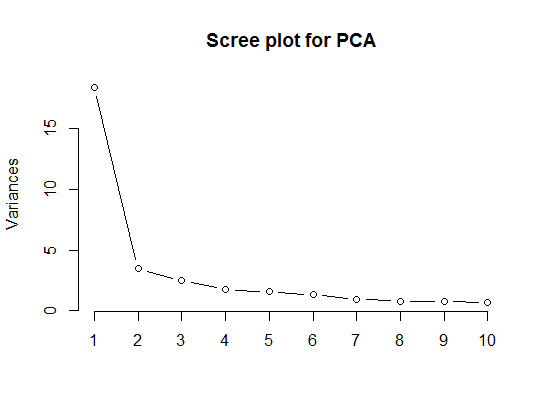
\includegraphics[width=3in]{scree.png}}}
\caption{Scree plot for PCA.}
\label{figurelabel}
\end{figure}

\begin{figure}[thpb]
\centering
\framebox{\parbox{3in}{
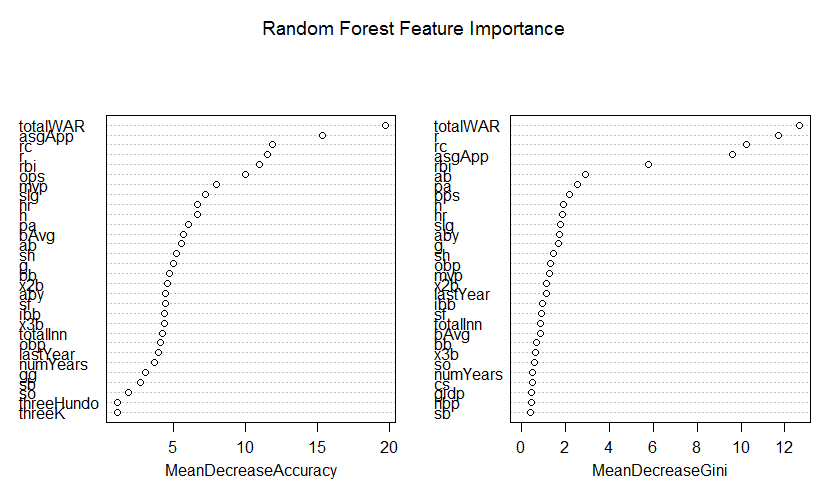
\includegraphics[width=3in]{rfImp.png}}}
\caption{Variable importance chart for random forest classifier.}
\label{figurelabel}
\end{figure}

\begin{figure}[thpb]
\centering
\framebox{\parbox{3in}{
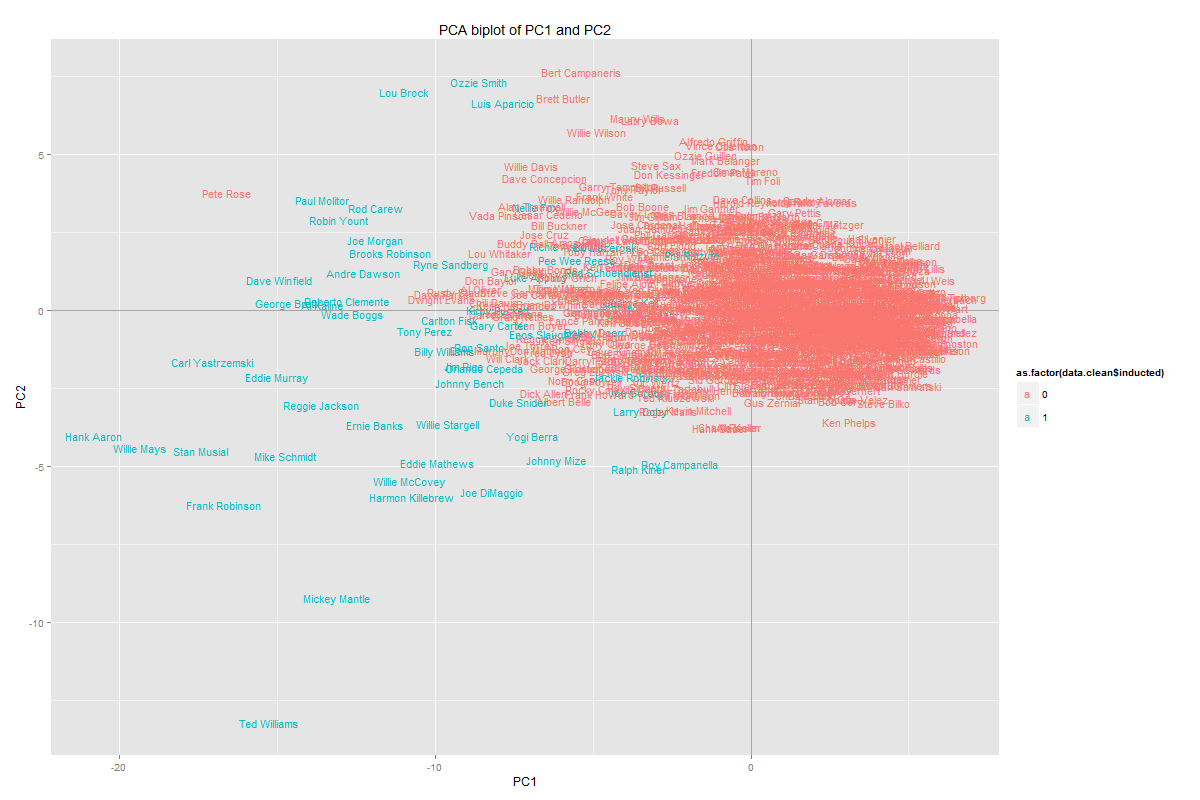
\includegraphics[width=3in]{pca2.png}}}
\caption{PCA biplot for modern batter dataset. Full size at https://github.com/stillmatic/baseball/blob/master/pca2.png}
\label{figurelabel}
\end{figure}

\section*{ACKNOWLEDGMENT}

Special thanks are due to Sean Lahman for his work in maintaining the Lahman Baseball Database. Additionally, Baseball Reference$'$s Wins Above Replacement data was invaluable for this analysis; making such data publicly available can only further benefit human knowledge. We would also like to thank Professor Zhao for her assistance in completing this project.

%%%%%%%%%%%%%%%%%%%%%%%%%%%%%%%%%%%%%%%%%%%%%%%%%%%%%%%%%%%%%%%%%%%%%%%%%%%%%%%%

\begin{thebibliography}{99}

\bibitem{c1} Cattell, R. B. (1966). The scree test for the number of factors. Multivariate Behavioral Research, pp 1, 629-637.
\bibitem{c2} Kaiser, H. F. (1960). The application of electronic computers to factor analysis. Educational and Psychological Measurement, 20, pp 141-151.
\bibitem{c3} Svetnik, V.; Liaw, A.; Tong, C. (2003) Random forest: a classification and regression tool for compound classification and QSAR modeling. Journal of Chemical Information and Modeling, 43 (6), pp 1947–1958.
\bibitem{c4} Gladwell, M. (2008). Outliers. Little, Brown and Company. 978-0-316-01792-3.
\bibitem{c5} Lewis, M. (2003). Moneyball: The Art of Winning an Unfair Game. W. W. Norton \& Company. 978-0-393-05765-2.
\bibitem{c6} Derman, E. (2007). My Life as a Quant: Reflections on Physics and Finance. Wiley. 978-0470192733.


\end{thebibliography}

\end{document}
